Рассмотрим описаные алгоритмы шифрования строки и конвейеризации.

\section{Алгоритмы шифрования}
Рассмотрим работу алгоритов шифрования. Пусть на вход подаётся строка $s$ длины $len$.

	\subsection{Шифр Фейстеля}
	Алгоритм циклически обходит пары рядом стоящих символов и производит для них $max_step$ итераций шифрования с помощью операции XOR.
	
	Схема алгоритма приведена на рисунке 2.1
	\begin{figure}[h]
		\begin{center}
			{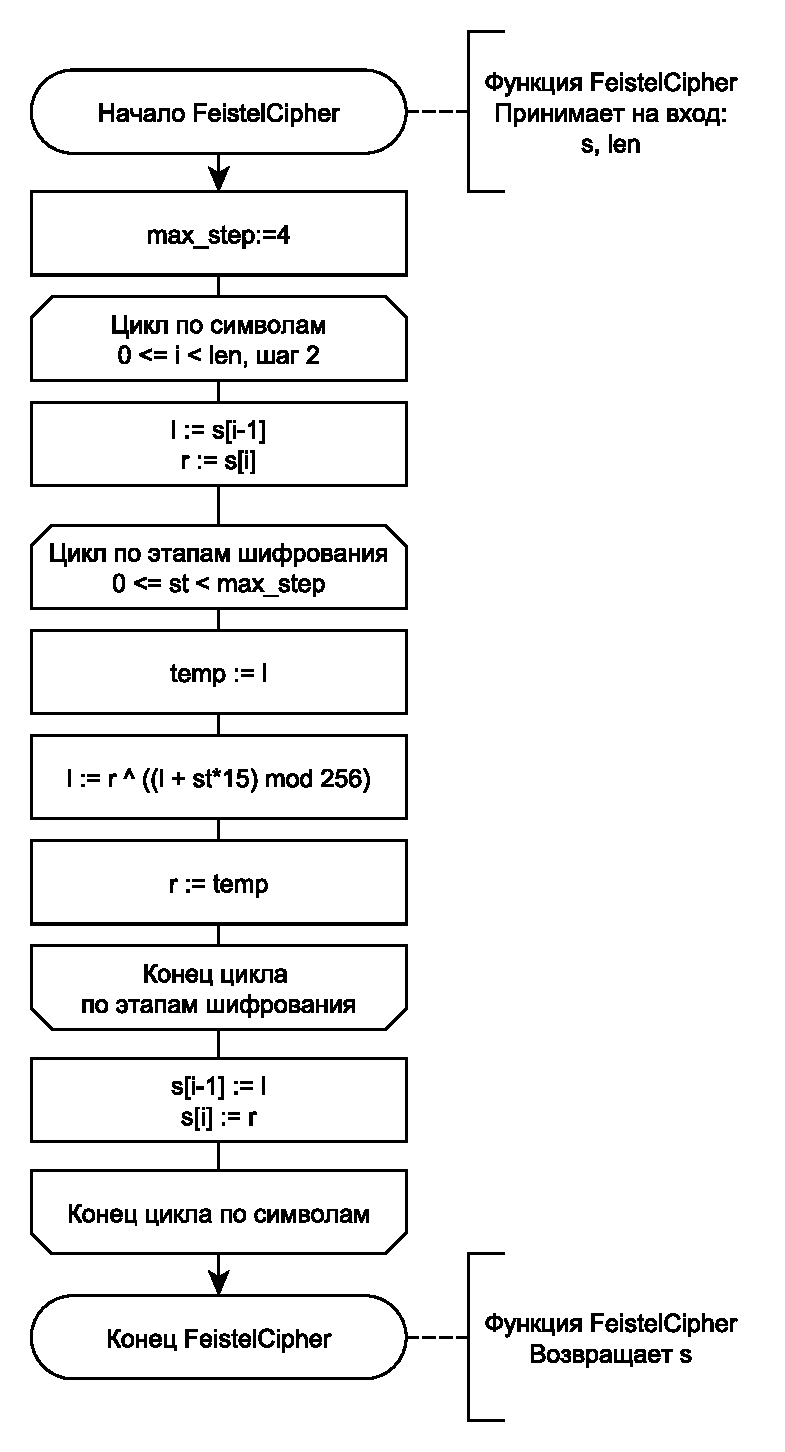
\includegraphics[height=20cm, width = 14cm]{Feistel}}
			\caption{Шифр Фейстеля}
		\end{center}
	\end{figure}


	\subsection{Шифр Тритемиуса}
	Алгоритм совершает цикл по всем символам строки и для каждого из них совершает вычисление нового значения символа в зависимости от исходнго и текущей позиции
	
	Схема алгоритма приведена на рисунке 2.2
	\begin{figure}[h]
		\begin{center}
			{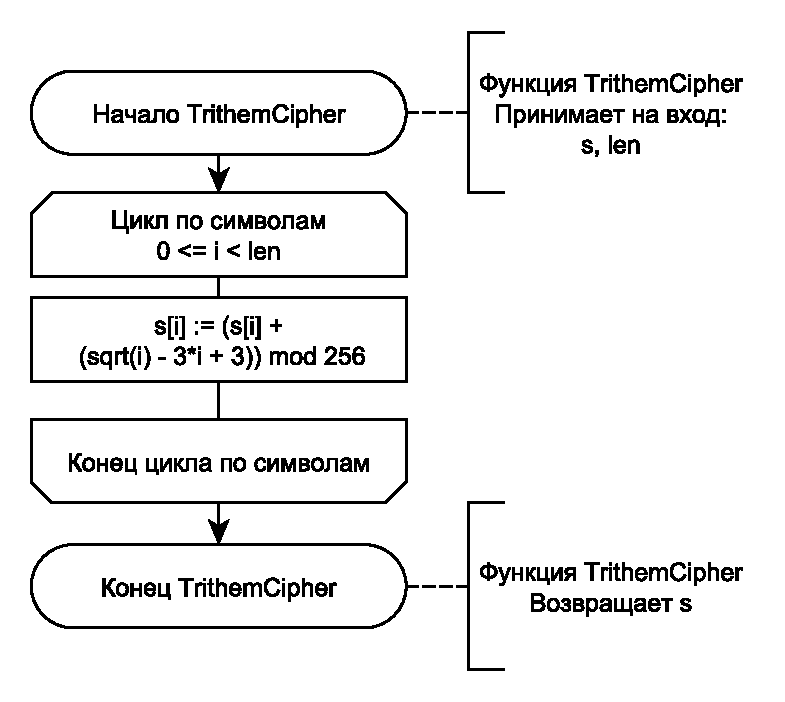
\includegraphics{Trithemius}}
			\caption{Шифр Тритемиуса}
		\end{center}
	\end{figure}


	\subsection{Шифр побитовыми сдвигами}
	Алгоритм производит циклический сдвиг вправо на $shift$ для $buf\_byte$ символов из строки s (с i-й позиции по i+buf\_byte), после чего переходит к следующему блоку данных увеличением i на 1.
	
	Схема алгоритма приведена на рисунке 2.3
	\begin{figure}[h]
		\begin{center}
			{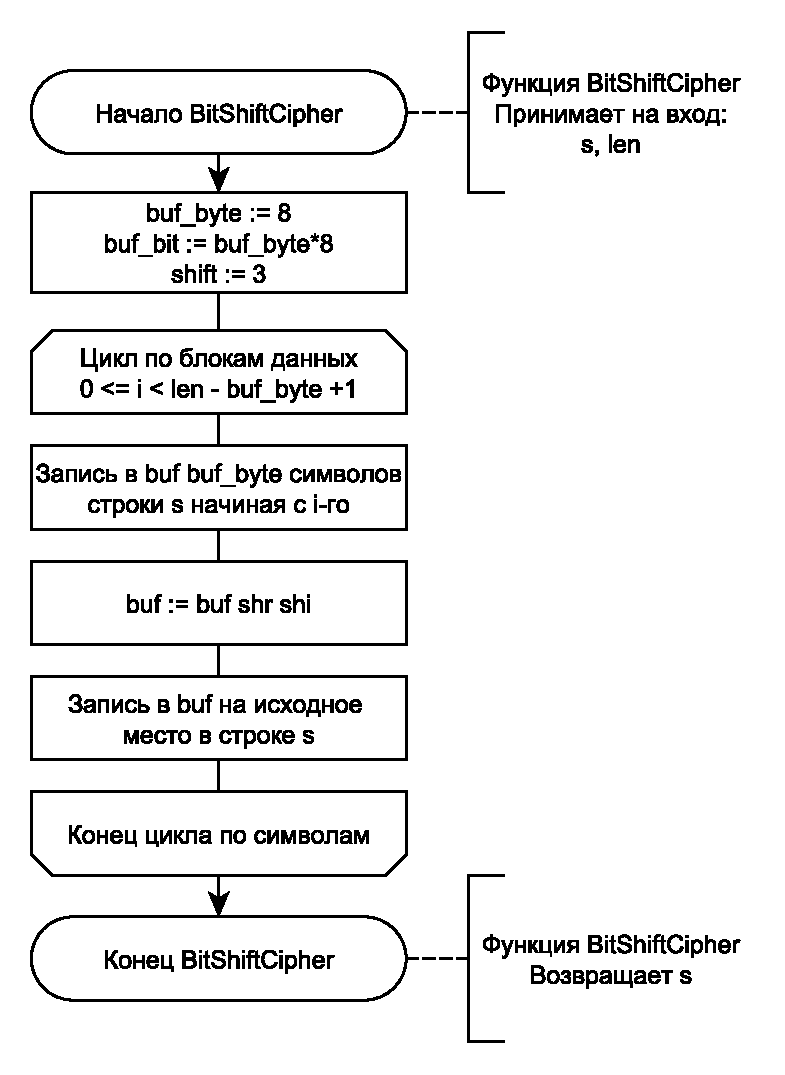
\includegraphics[height=20cm, width = 14cm]{BitShift}}
			\caption{Шифр побитовыми сдвигами}
		\end{center}
	\end{figure}


\section{Конвейеризация алгоритма}
Конвейеризация процесса происходит с помощью алгоритов работы для конвейера (главного потока) и его лент (рабочих потоков).

	\subsection{Алгоритм работы конвейера}
	Конвейер осуществляет заполнение входной очереди задачами. Задачи являются структурами имеющими в себе 6 полей для записи времени прихода/ухода с лент конвейера и сама задача в виде шифруемой строки. После заполнения, конвейер запускает в работу три ленты конвейера и ожидает их завершения. Дальше конвейер совершает обработку полученной статистики.
	
	Схема алгоритма приведена на рисунке 2.4
	\begin{figure}[h]
		\begin{center}
			{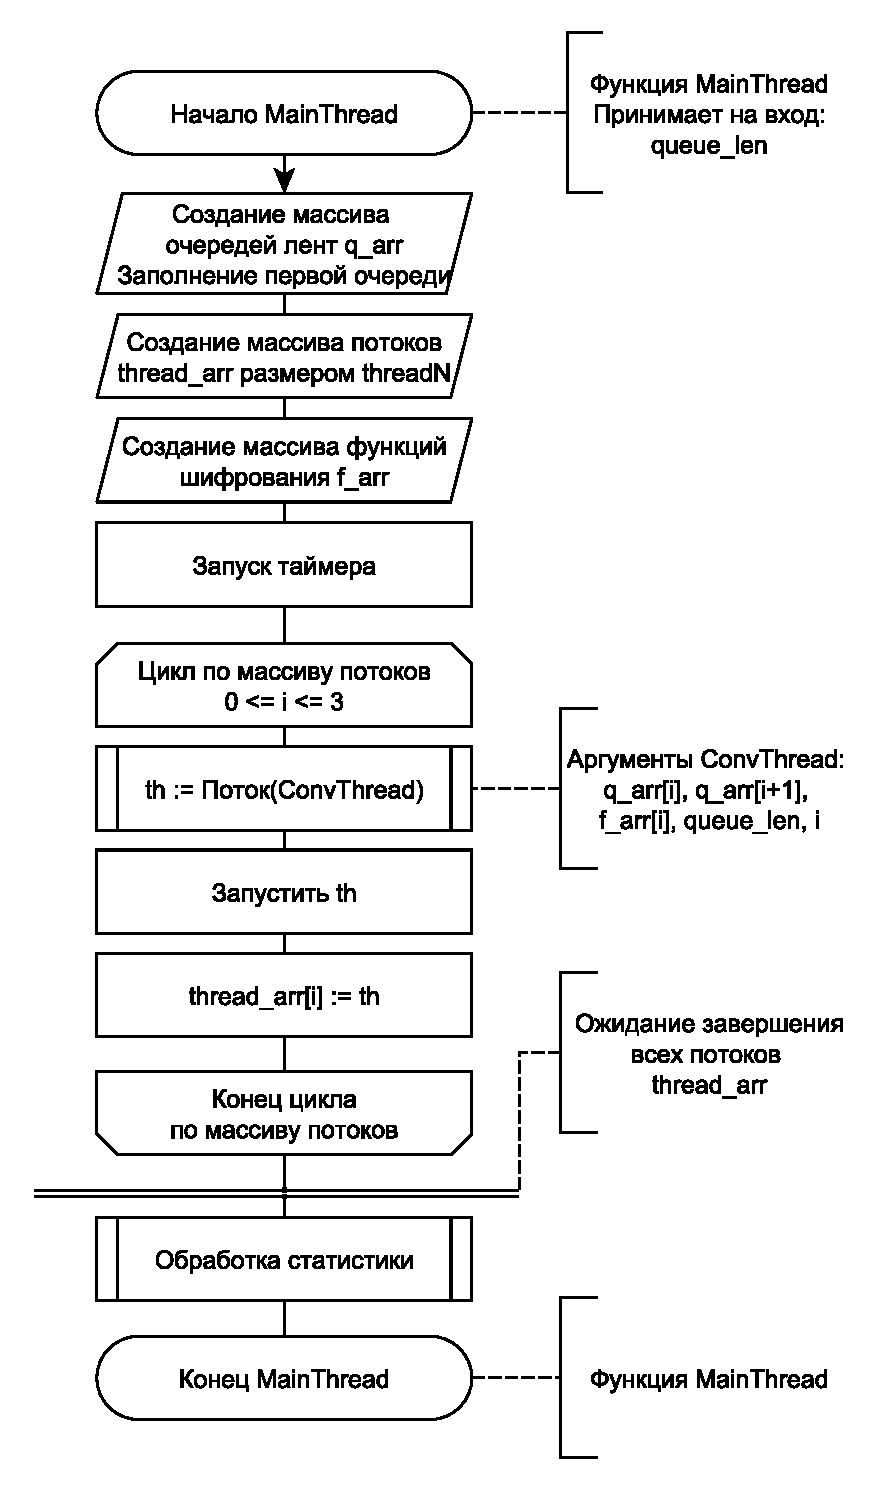
\includegraphics[height=20cm, width = 14cm]{Main}}
			\caption{Алгоритм работы конвейера}
		\end{center}
	\end{figure}

	\subsection{Алгоритм работы ленты}
	Лента производит обработку $queue\_len$ количества задач. В начале обработки происходит ожидание поступления очередной задачи во входную очередь, после чего она выталкивается из очереди в переменную задачи. Выполняется функция шифрования, записывается время начала и конца обработки. Обработанная структура записывается в выходную очередь
	
	Схема алгоритма приведена на рисунке 2.5
	\begin{figure}[h]
		\begin{center}
			{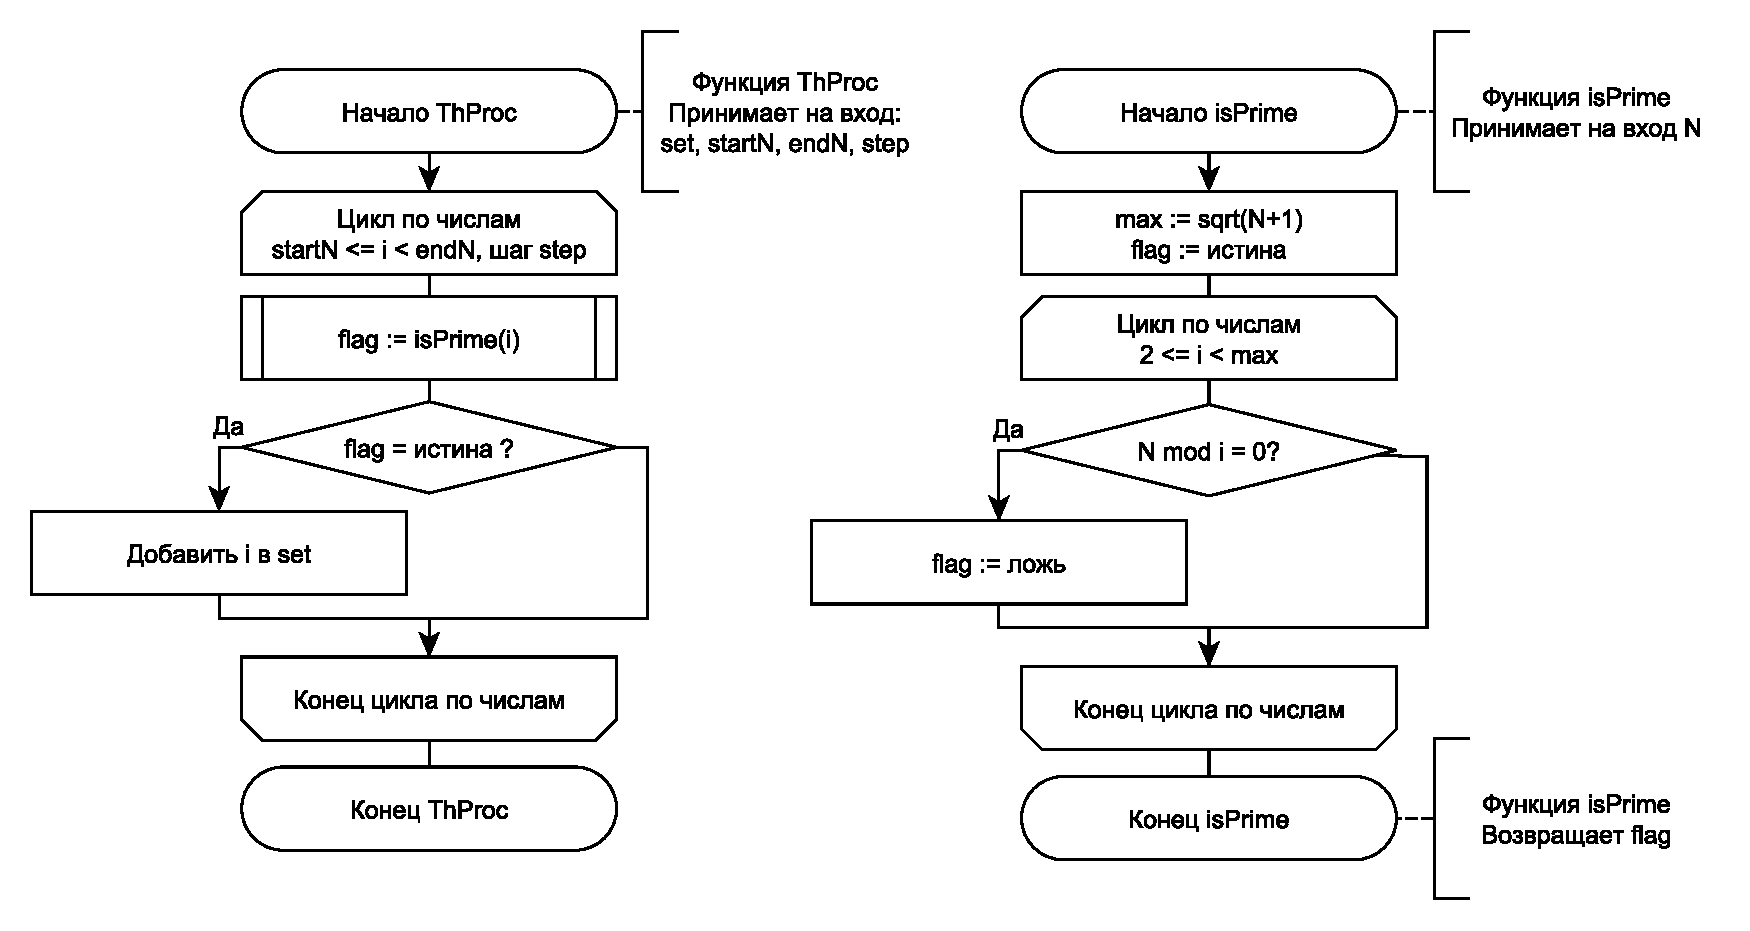
\includegraphics[height=20cm, width = 14cm]{Work}}
			\caption{Алгоритм работы ленты}
		\end{center}
	\end{figure}


\section{Требования к программному обеспечению}
Для полноценной проверки и оценки алгоритмов необходимо выполнить следующее.
\begin{enumerate}
	\item Предоставить возможность ввода количества задач.
	\item Реализовать функцую вывода информации о каждой обработанной задаче и функции подсчёта и вывода статистических данных.
	\item Реализовать функцию замера процессорного времени, затраченного функциями.
\end{enumerate}


\section{Заготовки тестов}
При проверке алгоритма необходимо будет использовать следующие классы тестов:
\begin{itemize}
	\item одна задача;
	\item 1000 задач.
\end{itemize}

\section*{Вывод}
Результатом конструторской части стало схематическое описание алгоритмов шифрования строк и конвейеризации алгоритма, сформулированны тесты и требования к программному обеспечению.

